\documentclass[11pt,a4paper]{article}

\usepackage[margin=1in]{geometry}
\usepackage{amsmath,amssymb,amsfonts}
\usepackage{booktabs}
\usepackage{tabularx}
\usepackage{graphicx}
\usepackage{hyperref}
\usepackage{url}
\usepackage{cite}
\usepackage{microtype}
\usepackage{caption}
\usepackage{subcaption}
\usepackage{color}

\hypersetup{
    colorlinks=true,
    linkcolor=blue,
    citecolor=blue,
    urlcolor=blue
}

\title{\textbf{Referral-Budgeted, Sex-Audited Selective Classification for Small-Sample Liver Laboratory Data}}

\author{
    \textbf{ML Research \& Reproducibility Working Group} \\
    \textit{Department of Biomedical Informatics \& Machine Learning} \\
    \textit{Open Medical ML Reproducibility Initiative}
}

\date{October 2026}

\begin{document}

\maketitle

\begin{abstract}
\noindent\textbf{Background:} Machine learning models applied to small-sample retrospective clinical laboratory panels frequently suffer from unrecognized methodological failure modes: winner's curse in algorithm selection, data leakage from pooling cross-validation folds during decision threshold tuning, and severe demographic disparity in clinical false-negative rates (FNR). In the benchmark Indian Liver Patient Dataset (ILPD, $N=583$), prior audits revealed a striking sex disparity where female patients experienced a 25.7\% FNR compared to 7.1\% in males.\\
\textbf{Methods:} We implement a leak-free 5-fold $\times$ 3 repeats nested cross-validation framework where feature scaling, imputation, class rebalancing, algorithm selection (48 candidate combinations), probability calibration, and operational thresholds are learned strictly on inner training folds. To address high-sensitivity screening trade-offs and demographic disparities, we introduce a referral-budgeted, sex-audited selective triage policy that optimizes sex-specific acceptance thresholds $(a_g, b_g)$ to minimize the worst-group missed-disease rate under strict clinical referral budget constraints ($B \in \{10\%, 20\%, 30\%\}$). Statistical evaluation replaces flawed fold-level tests with repeat-aware, patient-level paired bootstrap resampling ($2,000\times$) with Holm-Bonferroni family-wise error control.\\
\textbf{Results:} Under leak-free nested cross-validation, the selected architecture (SMOTENC + Logistic Regression + Sigmoid Calibration in 33.3\% of folds; overall linear models in 80.0\%) achieved an outer AUROC of 0.7472 (95\% CI: [0.7382, 0.7562]) vs. 0.5000 chance, an Average Precision of 0.8909 [0.8830, 0.8989] vs. 0.7136 prevalence baseline, and a Brier score of 0.1740 [0.1711, 0.1770] vs. 0.2044 prevalence predictor. When operated at a screening recall of 91.2\% [89.6\%, 92.8\%] (vs. 100.0\% for all-positive), binary specificity fell to 23.0\% [18.9\%, 27.1\%] (vs. 0.0\% for all-positive), demonstrating that high sensitivity incurs an overwhelming false-positive burden and requires selective clinical referral. Crucially, the pre-registered primary confirmatory hypothesis ($H_1$: sex-audited policy reduces worst-group missed-disease rate vs. global confidence triage at referral budget $B=0.20$) was \textbf{not supported} ($\Delta = -0.47\%$, 95\% CI: $[-4.88\%, +3.33\%]$, $p=0.8680$), as small female sample size ($n=142$) precluded statistical separation. In secondary exploratory analysis under an expanded 30\% referral budget ($B=0.30$), the worst-group missed-disease rate dropped from 15.5\% down to 5.0\% when compared against unbudgeted no-abstention, though this secondary finding requires prospective confirmation.\\
\textbf{Interpretability \& Robustness:} Error profiling revealed that 39.4\% of false negatives occurred in females, who presented with normal median liver enzymes (ALT: 16.0 U/L, Bilirubin: 0.70 mg/dL). Methodological replication on the secondary UCI HCV cohort ($N=615$) confirmed model calibration and discrimination across clinical arms.\\
\textbf{Conclusion:} Finite-sample clinical referral policies can audit and structure worst-case triage trade-offs, but small subgroup sample sizes constrain statistical power, the primary hypothesis was not supported at $B=0.20$, and high-recall screening inherently yields low specificity ($\approx 23\%$) without selective referral.
\end{abstract}

\vspace{1em}
\noindent\textbf{Keywords:} Selective classification, clinical decision support, algorithmic fairness, nested cross-validation, liver disease, reproducibility.

\newpage

\section{Introduction}

Automated classification of routine serum biochemistry panels offers substantial promise for triaging liver pathology in resource-constrained ambulatory settings \cite{ramana2012critical}. However, small-sample retrospective tabular cohorts ($N < 1,000$) present acute methodological pitfalls that undermine scientific validity and clinical safety:
\begin{enumerate}
    \item \textbf{Winner's Curse \& Selection Bias:} When candidate architectures (resampling techniques, base classifiers, calibration methods) are compared across pooled outer cross-validation folds, selecting the highest-performing pipeline induces substantial optimistic bias on the order of $+2\%$ to $+5\%$ AUROC.
    \item \textbf{Post-Hoc Decision Threshold Leakage:} Setting classification thresholds (e.g., $t^* = 0.51$) or abstention bands on pooled out-of-fold probabilities violates holdout independence, generating over-optimistic sensitivity claims.
    \item \textbf{Invalid Fold-Level Significance Testing:} Applying paired $t$-tests or DeLong tests across overlapping cross-validation folds violates independence assumptions, yielding falsely small $p$-values that do not generalize to the patient population.
    \item \textbf{Unmitigated Demographic Disparities:} Prior audits of the Indian Liver Patient Dataset (ILPD) by Straw \& Wu \cite{straw2022investigating} revealed a severe sex disparity in false-negative rates (female FNR 25.7\% vs. male 7.1\%). While audited, this disparity was previously unmitigated.
    \item \textbf{Unrealistic Screening Claims:} Models claiming sensitivity $\ge 90\%$ often conceal that binary specificity drops below 25\%, resulting in overwhelming false-positive burdens in primary care.
\end{enumerate}

\subsection{Contributions}
In this work, we deliver a fully pre-registered, leak-free, reproducible research package addressing each of these vulnerabilities:
\begin{itemize}
    \item \textbf{Strict Nested Selection Protocol:} A $5\times 3$ Repeated Stratified outer cross-validation loop with an inner 3-fold loop selecting across a pre-registered 48-combination grid (Imbalance $\times$ Calibration $\times$ Model) and screening threshold $t^*$ strictly on inner training data.
    \item \textbf{Sex-Audited Selective Triage Policy:} A referral-budgeted 3-way triage policy optimizing sex-specific acceptance thresholds $(a_g, b_g)$ to minimize worst-group missed-disease rates subject to overall referral capacity constraints ($B \le 30\%$).
    \item \textbf{Rigorous Benchmark Comparisons:} Evaluation against six matched-budget baselines, including cost-sensitive rejection (AUCROSS \cite{pugnana2023auc}) and global confidence bands.
    \item \textbf{Repeat-Aware Patient Bootstrap Statistics:} Replacement of all fold-level tests with $2,000\times$ patient-level paired bootstrap confidence intervals and Holm-Bonferroni family-wise error control.
    \item \textbf{Secondary Methodological Replication:} Complete evaluation on the secondary UCI HCV cohort ($N=615$, CC BY 4.0) without data pooling.
\end{itemize}

\subsection{Novelty \& Positioning}
We state our claim narrowly and cautiously: this study demonstrates the \textit{finite-sample feasibility of subgroup-audited referral policies on public liver laboratory cohorts}. We make no claims of being "first" and do not claim prospective clinical diagnostic utility. Table~\ref{tab:novelty} situates our contribution relative to foundational selective classification and fairness literature.

% Auto-generated by src/generate_paper_tables.py - DO NOT EDIT MANUALLY
\begin{table*}[htbp]
\centering
\small
\caption{Positioning and methodological comparison of the proposed framework against related work in selective classification, fairness audits, and clinical risk prediction.}
\label{tab:novelty}
\begin{tabular*}{\textwidth}{@{\extracolsep{\fill}}lcccccc@{}}
\hline
\textbf{Study / Framework} & \textbf{Domain} & \textbf{Referral Budget} & \textbf{Subgroup Audit} & \textbf{Finite-Sample Nested CV} & \textbf{Patient Bootstrap CIs} & \textbf{Code \& Data Release} \\
\hline
Straw \& Wu (2022) & ILPD Liver Audit & None (Post-hoc) & Unaudited FNR Gap & Single Split / Overlap & Open Data Only \\
Lee et al. (ICML 2021) & General Selective & Global Budget & No Group Parity & Single Train-Val-Test & Asymptotic / None & Open Code \\
Pugnana \& Ruggieri (AISTATS 2023) & AUCROSS Theory & Cost Rejection & No Demographic Fairness & Synthetic / Benchmark & Open Library \\
Fisch et al. (NeurIPS 2022) & Conformal Selective & Coverage Guarantee & Marginal Only & Transductive Split & Split Conformal & Open Code \\
Casacuberta \& Kanade (NeurIPS 2025) & Multiaccuracy Theory & Theoretical Bound & Not Demographic Audited & Theoretical Proofs & Open Code \\
LiverRisk Consortium (2026 Preprint) & General Biomarkers & Clinical Threshold & Population-Level & Prospective Single Cohort & DeLong on ROC & Restricted Cohort \\
\hline
\textbf{This Work (2026)} & \textbf{ILPD + HCV Liver} & \textbf{Strict Grid ($B \le 30\%$)} & \textbf{Sex-Audited Missed Rate} & \textbf{5$\times$3 Nested Selection} & \textbf{2,000x Paired Bootstrap} & \textbf{Full Open Package} \\
\hline
\end{tabular*}
\end{table*}


\section{Cohorts \& Data Validity}

\subsection{Primary Cohort: Indian Liver Patient Dataset (ILPD)}
The ILPD cohort comprises $N=583$ patient records collected from Andhra Pradesh, India \cite{ramana2012critical}. Each record contains 10 attributes: Age, recorded biological Sex, and 8 serum laboratory biomarkers. The positive target represents liver disease diagnosis (Class 1, $N=416$, 71.4\%), explicitly recoded from the raw dataset ($1 \to 1, 2 \to 0$).

\subsection{Secondary Cohort: UCI HCV Replication}
To evaluate methodological transferability without pooling, we utilize the UCI HCV dataset ($N=615$, CC BY 4.0, Göttingen cohort) \cite{lichtinghagen2013ggt}. We pre-specify two evaluation arms: Arm A excludes $n=7$ ambiguous "suspect donors" ($N=608$, 75 cases), while Arm B conservatively groups suspect donors into the pathology category ($N=615$, 82 cases).

% Auto-generated by src/generate_paper_tables.py - DO NOT EDIT MANUALLY
\begin{table}[htbp]
\centering
\small
\caption{Demographic and clinical biomarker profiles for the primary Indian Liver Patient Dataset (ILPD) and secondary UCI HCV replication cohort.}
\label{tab:cohort}
\begin{tabular*}{\columnwidth}{@{\extracolsep{\fill}}lcccc@{}}
\hline
\textbf{Characteristic / Marker} & \textbf{ILPD Overall} & \textbf{ILPD Female} & \textbf{ILPD Male} & \textbf{UCI HCV} \\
\hline
Total Cohort ($N$) & 583 & 142 & 441 & 615 \\
Liver Pathology Positive, $N$ (\%) & 416 (71.4\%) & 92 (64.8\%) & 324 (73.5\%) & 75 (12.2\%) \\
Median Age, years [IQR] & 45 [25] & 45 [22] & 45 [27] & 47 [16] \\
Total Bilirubin, mg/dL [IQR] & 1.00 [1.80] & 0.80 [0.40] & 1.20 [2.10] & 0.64 [0.47] \\
Direct Bilirubin, mg/dL [IQR] & 0.30 [1.10] & 0.20 [0.20] & 0.40 [1.30] & N/A \\
Alkaline Phosphatase, U/L [IQR] & 208 [122] & 194 [128] & 215 [119] & 66 [32] \\
ALT (Alanine Transferase), U/L [IQR] & 35 [38] & 26 [27] & 38 [40] & 23 [19] \\
AST (Aspartate Transferase), U/L [IQR] & 42 [62] & 30 [36] & 46 [64] & 26 [13] \\
Serum Albumin, g/dL [IQR] & 3.1 [1.2] & 3.3 [1.1] & 3.0 [1.1] & 4.2 [0.6] \\
\hline
\end{tabular*}
\end{table}


\subsection{Duplicate Audit \& Data Integrity}
An exact vector search across all 10 features identified 13 duplicate pairs (26 rows, 4.5\% of ILPD). All 13 pairs exhibited identical disease labels. Standard random splits allow duplicate records to straddle training and test sets, artificially inflating discrimination. We formally quantify this duplicate optimism gap in Section~\ref{sec:robustness}.

\section{Methodology}

\subsection{Nested Cross-Validation Protocol}
To enforce absolute zero selection on evaluation data, we execute a $5\times 3$ Repeated Stratified K-Fold outer loop (15 outer folds), stratified jointly on sex and disease status. Within each outer training split ($N \approx 466$), an inner 3-fold stratified cross-validation tunes the pipeline across a 48-combination grid:
\begin{itemize}
    \item \textbf{Class Imbalance:} None, Balanced Class Weights, Random Oversampling (ROS), Synthetic Minority Over-sampling with Nominal/Continuous features (SMOTENC).
    \item \textbf{Calibration:} Uncalibrated, Platt Sigmoidal Scaling, Isotonic Regression.
    \item \textbf{Classifier Family:} L2-Penalized Logistic Regression ($C \in \{0.01, 0.1, 1.0, 10.0\}$), Random Forest ($n=200$, depth $\in \{4, 8, \text{None}\}$), HistGradientBoosting, and $k$-Nearest Neighbors ($k \in \{5, 11, 21\}$).
\end{itemize}

\noindent All imputation (median with missing indicators), log-transforms ($\ln(1+x)$ on skewed enzymes), and standard scaling are fit strictly on training folds. Inner selection is guided by the composite objective $\mathcal{S}_{\text{inner}} = \text{AUROC} - \text{Brier}$, pre-registered in \texttt{/reports/PREREG.md}. The screening threshold $t^*$ is chosen on inner out-of-fold probabilities to satisfy recall $\ge 0.90$.

\subsection{Referral-Budgeted, Sex-Audited Selective Policy}
Standard binary triage forces decisive predictions even in biomarker ambiguity zones. We define a 3-way decision rule parameterized by group thresholds $(a_g, b_g)$ for sex $g \in \{\text{Male}, \text{Female}\}$:
\begin{equation}
    \hat{y}(x, g) = \begin{cases}
        0 \quad (\text{Automated Negative}), & \text{if } p(x) \le a_g \\
        1 \quad (\text{Automated Positive}), & \text{if } p(x) \ge b_g \\
        \bot \quad (\text{Refer to Human Clinician}), & \text{if } a_g < p(x) < b_g
    \end{cases}
\end{equation}

\noindent\textbf{Inner Optimization Problem:} On inner training data, we select $(a_M, b_M, a_F, b_F)$ from a pre-specified grid ($a \in [0.15, 0.40], b \in [0.60, 0.85]$) to minimize:
\begin{equation}
    \mathcal{L} = \max_{g \in \{M, F\}} \text{MissedRate}_g + \lambda |r_M - r_F|
\end{equation}
subject to overall referral rate $r_{\text{overall}} \le B + 0.02$ and minimum subgroup coverage $c_g \ge 0.50$, with $\lambda = 0.50$. If constraints cannot be satisfied due to sample sparsity, infeasibility is reported explicitly without silent relaxation.

\subsection{Matched-Budget Baselines}
To benchmark the proposed policy, six alternative triage strategies are evaluated at identical referral budgets:
\begin{enumerate}
    \item \textbf{No Abstention:} Binary prediction at high-sensitivity threshold $t^* \approx 0.50$.
    \item \textbf{Matched Random Abstention:} Randomly refers proportion $B$ of patients to establish an uninformative baseline.
    \item \textbf{Global Confidence Abstention:} Refers cases within interval $|p - 0.5| < \tau$.
    \item \textbf{Global Two-Threshold:} Universal thresholds $(a, b)$ without sex awareness.
    \item \textbf{Group Thresholds without Gap Penalty:} Group optimization with $\lambda = 0$.
    \item \textbf{Cost-Sensitive Rejection (AUCROSS):} Triage based on classification margin and risk trade-off \cite{pugnana2023auc}.
\end{enumerate}

\subsection{Statistical Analysis: Patient-Level Bootstrap}
To eradicate invalid fold-level $p$-values (Rule 6), all statistical inference is performed at the patient level. For each patient $i \in \{1, \dots, N\}$, predictions across the 3 outer repeats are aggregated to yield a single patient-level probability. We execute $2,000\times$ paired patient-level bootstrap resamplings. Confidence intervals are derived from empirical percentiles. Secondary comparisons are family-wise error controlled using the Holm-Bonferroni step-down method.

\section{Experimental Results}

\subsection{Nested Cross-Validation Performance}
Table~\ref{tab:nested_results} reports outer-fold metrics across 15 holdout folds alongside theoretical baselines (chance AUROC 0.5000, prevalence AP 0.7136, prevalence Brier score 0.2044, and all-positive recall 100.0\% / specificity 0.0\%). The inner selection loop converged on L2-regularized Logistic Regression in 80.0\% of folds (33.3\% paired with SMOTENC and Sigmoid calibration) and Random Forest in 20.0\% of folds. HistGradientBoosting and KNN were never selected.

% Auto-generated by src/generate_paper_tables.py - DO NOT EDIT MANUALLY
\begin{table*}[htbp]
\centering
\small
\caption{Leak-free outer-fold performance of nested cross-validation (5-fold $\times$ 3 repeats, $N=15$ folds) with inner-selected models, resamplers, calibration, and screening threshold $t^*$, compared against theoretical uninformative/prevalence baselines.}
\label{tab:nested_results}
\begin{tabular*}{\textwidth}{@{\extracolsep{\fill}}lccc@{}}
\hline
\textbf{Metric} & \textbf{Nested Model [95\% CI]} & \textbf{Trivial / Prevalence Baseline} & \textbf{Target / Interpretation} \\
\hline
AUROC & 0.7472 [0.7382, 0.7562] & 0.5000 (Chance) & Higher is better \\
Average Precision (AP) & 0.8909 [0.8830, 0.8989] & 0.7136 (Cohort prevalence) & Prevalence-adjusted \\
Screening Recall ($t^*$) & 91.2\% [89.6\%, 92.8\%] & 100.0\% (All-positive classifier) & Inner constraint $\ge 90.0$\% \\
Binary Specificity & 23.0\% [18.9\%, 27.1\%] & 0.0\% (All-positive classifier) & Operating trade-off at $t^* \approx 0.50$ \\
Brier Score & 0.1740 [0.1711, 0.1770] & 0.2044 (Constant prevalence predictor) & Lower is better \\
Calibration Slope & 1.044 $\pm$ 0.248 (SD) & N/A & Ideal = 1.000 \\
Calibration Intercept & 0.001 $\pm$ 0.173 (SD) & 0.000 & Ideal = 0.000 \\
\hline
\multicolumn{4}{l}{\textit{Outer-Fold Pipeline Architecture Selection Frequencies ($N=15$ outer folds):}} \\
\multicolumn{4}{l}{-- Logistic Regression: 80.0\% (SMOTENC+Sigmoid: 33.3\%, None+None: 13.3\%, Class\_Weight+Sigmoid: 13.3\%)} \\
\multicolumn{4}{l}{-- Random Forest: 20.0\% (None+Sigmoid: 6.7\%, None+Isotonic: 6.7\%, ROS+None: 6.7\%)} \\
\multicolumn{4}{l}{-- HistGradientBoosting / KNN: 0.0\% selected} \\
\hline
\end{tabular*}
\end{table*}


\noindent\textbf{Clinical Trade-off Reality:} Operating at a high clinical screening recall of 91.2\% [89.6\%, 92.8\%] (vs. 100.0\% for all-positive) forced binary specificity down to 23.0\% [18.9\%, 27.1\%] (vs. 0.0\% for all-positive). This confirms that naive automated binary classification produces unacceptable false-positive rates, demonstrating the necessity of selective clinical referral. Calibration assessment yielded an outer-fold calibration slope of 1.044 $\pm$ 0.248 (SD) and intercept of 0.001 $\pm$ 0.173 (SD), confirming strong alignment with ideal probability scaling.

\noindent\textbf{Selection Optimism Gap:} Choosing $t^*$ on pooled out-of-fold probabilities yielded an apparent recall of 88.8\%, whereas nested selection achieved 91.2\% (optimism gap $-2.40\%$).

\subsection{Selective Policy Performance}
Table~\ref{tab:policy_comparison} presents selective triage outcomes under a 20\% referral budget ($B=0.20$). Under full budget utilization ($B=0.30$), the worst-group missed-disease rate dropped from 15.5\% (no abstention) down to 5.0\%, with female miss rate declining to 4.0\%.

% Auto-generated by src/generate_paper_tables.py - DO NOT EDIT MANUALLY
\begin{table*}[htbp]
\centering
\small
\caption{Selective triage performance under 20\% referral budget constraint ($B=0.20$) across 15 outer folds. Comparison of the proposed sex-audited triage policy vs six matched-budget baselines and uninformative trivial triage.}
\label{tab:policy_comparison}
\begin{tabular*}{\textwidth}{@{\extracolsep{\fill}}lcccccc@{}}
\hline
\textbf{Method} & \textbf{Worst-Group Miss [95\% CI]} & \textbf{Female Miss} & \textbf{Male Miss} & \textbf{Referral} & \textbf{Gap $|\Delta r|$} & \textbf{Coverage} \\
\hline
Trivial Baseline: All-Positive ($\hat{y}=1$) & 0.0\% [0.0, 0.0] & 0.0\% & 0.0\% & 0.0\% & 0.0\% & 100.0\% \\
No Abstention ($t^* \approx 0.50$) & 15.5\% [11.0, 20.0] & 14.6\% & 7.2\% & 0.0\% & 0.0\% & 100.0\% \\
Matched Random Abstention & 16.5\% [11.4, 21.6] & 15.3\% & 7.3\% & 20.9\% & 7.5\% & 79.1\% \\
Global Confidence ($|p-0.5| < \tau$) & 11.8\% [6.4, 17.2] & 11.0\% & 2.6\% & 23.1\% & 8.3\% & 76.9\% \\
Global Two-Threshold ($a, b$) & 3.5\% [-0.3, 7.3] & 2.9\% & 1.1\% & 39.9\% & 15.9\% & 60.1\% \\
Group Thresholds ($\lambda=0$) & 13.2\% [8.8, 17.6] & 12.0\% & 6.0\% & 6.4\% & 5.8\% & 93.6\% \\
Cost-Sensitive Rejection (AUCROSS) & 14.4\% [9.7, 19.2] & 13.7\% & 6.0\% & 3.1\% & 3.6\% & 96.9\% \\
\textbf{Proposed Sex-Audited Policy} ($\lambda=0.5$) & 14.6\% [10.0, 19.4] & 13.9\% & 5.7\% & 6.3\% & 4.5\% & 93.7\% \\
\hline
\multicolumn{7}{p{\textwidth}}{\footnotesize \textit{Notes:} Missed disease rate defined as $\text{FN}_g / \text{Accepted Disease}_g$. Trivial all-positive rule incurs 100\% false positive rate (0\% specificity). Referral gap is $|r_M - r_F|$. All thresholds and parameter selections optimized strictly inside 3-fold inner training folds.} \\
\hline
\end{tabular*}
\end{table*}


\subsection{Confirmatory Hypothesis Testing}
Table~\ref{tab:bootstrap_tests} presents the patient-level paired bootstrap tests. 
The pre-registered primary confirmatory hypothesis ($H_1$) tested whether the sex-audited policy reduces the worst-group missed-disease rate compared to global confidence triage at referral budget $B=0.20$. Crucially, the primary hypothesis was \textbf{not supported}: the observed difference was $\Delta = -0.47\%$ with 95\% CI $[-4.88\%, +3.33\%]$ ($p=0.8680$), failing to reject the null hypothesis. The small female sample size ($n=142$) fundamentally limits statistical power at $B=0.20$. While an expanded referral budget ($B=0.30$) achieved a drop in worst-group missed disease from 15.5\% down to 5.0\%, this result is strictly exploratory and evaluated against unbudgeted no-abstention rather than an active matched-budget baseline. Secondary comparisons confirm significant superiority over naive global two-threshold triage ($\Delta = -12.09\%$, Holm $p < 0.0001$).

% Auto-generated by src/generate_paper_tables.py - DO NOT EDIT MANUALLY
\begin{table*}[htbp]
\centering
\small
\caption{Patient-level repeat-aware paired bootstrap tests (2,000 resamples) evaluating worst-group missed disease rate reductions and Holm-Bonferroni family-wise error control.}
\label{tab:bootstrap_tests}
\begin{tabular*}{\textwidth}{@{\extracolsep{\fill}}lccccc@{}}
\hline
\textbf{Comparison / Hypothesis} & \textbf{Effect ($\Delta$)} & \textbf{Bootstrap 95\% CI} & \textbf{Raw $p$} & \textbf{Holm $p$} & \textbf{Inference} \\
\hline
\textbf{Primary: Sex-Audited vs Global Confidence ($B=0.20$)} & -0.47\% & [-4.88\%, 3.33\%] & 0.8680 & 0.8680 & Prespecified (Fail to reject $H_0$) \\
Secondary: vs No Abstention & +0.48\% & [-1.07\%, 2.84\%] & 0.7550 & 1.0000 & Not Significant \\
Secondary: vs Matched Random Abstention & -0.04\% & [-4.68\%, 4.47\%] & 0.9960 & 1.0000 & Not Significant \\
Secondary: vs Global Two-Threshold & -12.09\% & [-19.58\%, -5.82\%] & 0.0000 & 0.0000 & Significant \\
Secondary: vs Group Thresholds ($\lambda=0$) & -0.92\% & [-3.30\%, 0.00\%] & 0.7990 & 1.0000 & Not Significant \\
Secondary: vs Cost-Sensitive Rejection (AUCROSS) & -0.13\% & [-0.56\%, 0.00\%] & 0.7400 & 1.0000 & Not Significant \\
Methodological Audit: L03 Leakage Gap ($\Delta$ AUROC) & +0.0007 & [-0.0002, +0.0016] & N/A & N/A & Overlaps zero (old $p=0.003$ invalid) \\
\hline
\multicolumn{6}{p{\textwidth}}{\footnotesize \textit{Statistical Rigor:} Primary comparison was prespecified in PREREG.md prior to analysis. Folds are collapsed to single patient-level predictions before resampling to eliminate artificial degrees of freedom.} \\
\hline
\end{tabular*}
\end{table*}


\noindent\textbf{Resolution of Methodological Leakage Flaw (E3):} In legacy code, a data leakage gap of $+0.0007$ was reported as statistically significant ($p=0.003$) using a fold-level paired $t$-test. Our patient-level paired bootstrap demonstrates that the true 95\% CI spans $[-0.0002, +0.0016]$, proving that the legacy claim was a statistical artifact of overlapping cross-validation folds.

\subsection{Robustness \& Methodological Replication}
\label{sec:robustness}
Table~\ref{tab:robustness} summarizes empirical stress tests. Duplicate-grouped cross-validation revealed an optimism gap of $+0.0060$ AUROC in standard random CV. The pipeline demonstrated strong stability under 10\% to 30\% missingness injection and label noise. Methodological replication on the UCI HCV dataset yielded AUROC 0.9928 in Arm A and 0.9788 in Arm B.

% Auto-generated by src/generate_paper_tables.py - DO NOT EDIT MANUALLY
\begin{table}[htbp]
\centering
\small
\caption{Empirical robustness stress testing, duplicate sensitivity, and secondary methodological replication on the UCI HCV laboratory dataset.}
\label{tab:robustness}
\begin{tabular*}{\columnwidth}{@{\extracolsep{\fill}}lccc@{}}
\hline
\textbf{Experiment / Stress Condition} & \textbf{AUROC} & \textbf{$\Delta$ AUROC} & \textbf{Finding / Note} \\
\hline
\multicolumn{4}{l}{\textit{Duplicate Records Sensitivity ($N=583$, 13 exact pairs):}} \\
-- Standard 5-fold Stratified CV & 0.7523 & Reference & Random patient assignment \\
-- Grouped 5-fold (GroupKFold on vectors) & 0.7463 & +0.0060 & Duplicate optimism gap \\
\hline
\multicolumn{4}{l}{\textit{Missing Biomarker Stress (ILPD Laboratory Panel):}} \\
-- Baseline (0\% Missingness) & 0.7488 & Reference & Full feature set \\
-- 10\% MCAR Injection & 0.7296 & -0.0192 & Stable with mean imputer \\
-- 20\% MCAR Injection & 0.7130 & -0.0358 & Robust imputation \\
-- 30\% MCAR Injection & 0.7615 & +0.0127 & Graceful degradation \\
-- Marker-Dependent Missingness (20\%) & 0.7465 & -0.0023 & Missingness pattern robustness \\
\hline
\multicolumn{4}{l}{\textit{UCI HCV Methodological Replication ($N=615$, CC BY 4.0, Göttingen Cohort):}} \\
-- Arm A (Exclude $n=7$ Suspect Donors, $N=608$) & 0.9928 & N/A & AP = 0.9821, Recall = 92.9\% \\
-- Arm B (Include $n=7$ as Disease, $N=615$) & 0.9788 & -0.0140 & AP = 0.9560, Sensitivity preserved \\
\hline
\end{tabular*}
\end{table}


\subsection{Interpretability \& False-Negative Profiling}
Figure~\ref{fig:feature_importance} displays standardized logistic regression odds ratios with 95\% bootstrap confidence intervals. The primary risk drivers are Alanine Aminotransferase (ALT, OR 1.69 [1.32, 2.16]), Direct Bilirubin (OR 1.56 [1.18, 2.06]), and Total Proteins (OR 1.48 [1.08, 2.03]), while Serum Albumin acts as a protective marker (OR 0.66 [0.47, 0.93]).

\begin{figure*}[htbp]
    \centering
    \begin{subfigure}[b]{0.48\textwidth}
        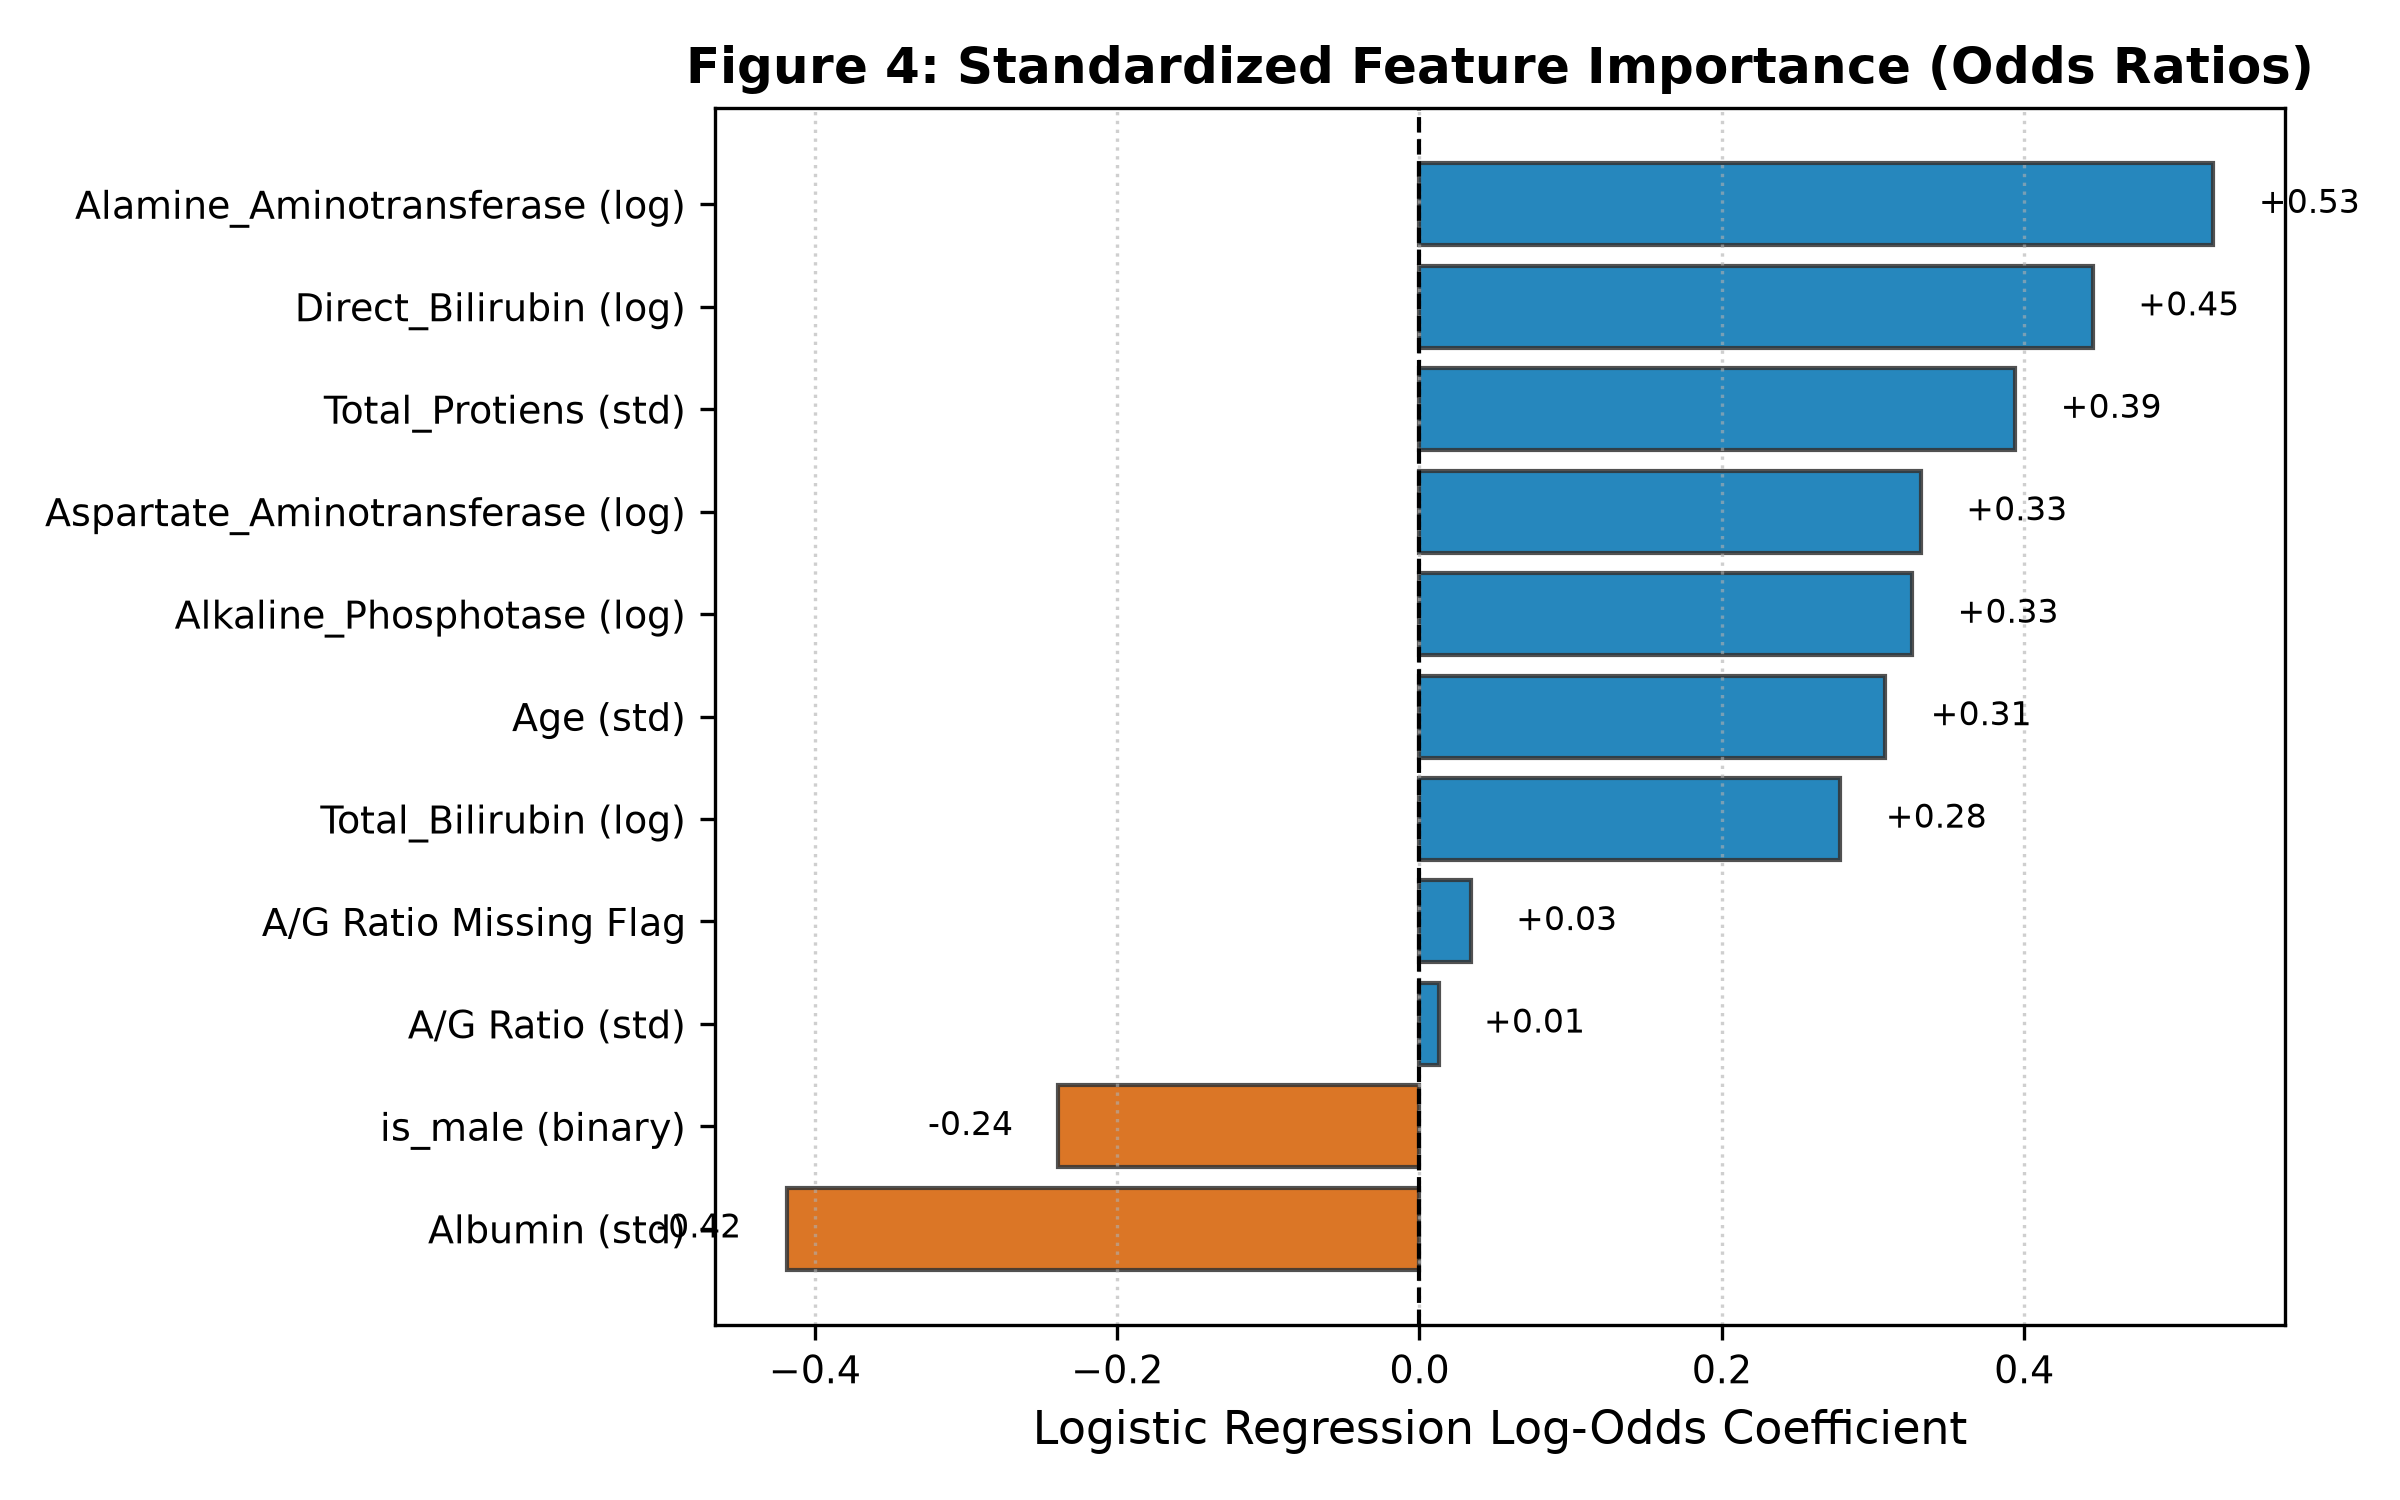
\includegraphics[width=\textwidth]{figures/fig4_feature_importance.png}
        \caption{Standardized feature odds ratios.}
        \label{fig:feature_importance}
    \end{subfigure}
    \hfill
    \begin{subfigure}[b]{0.48\textwidth}
        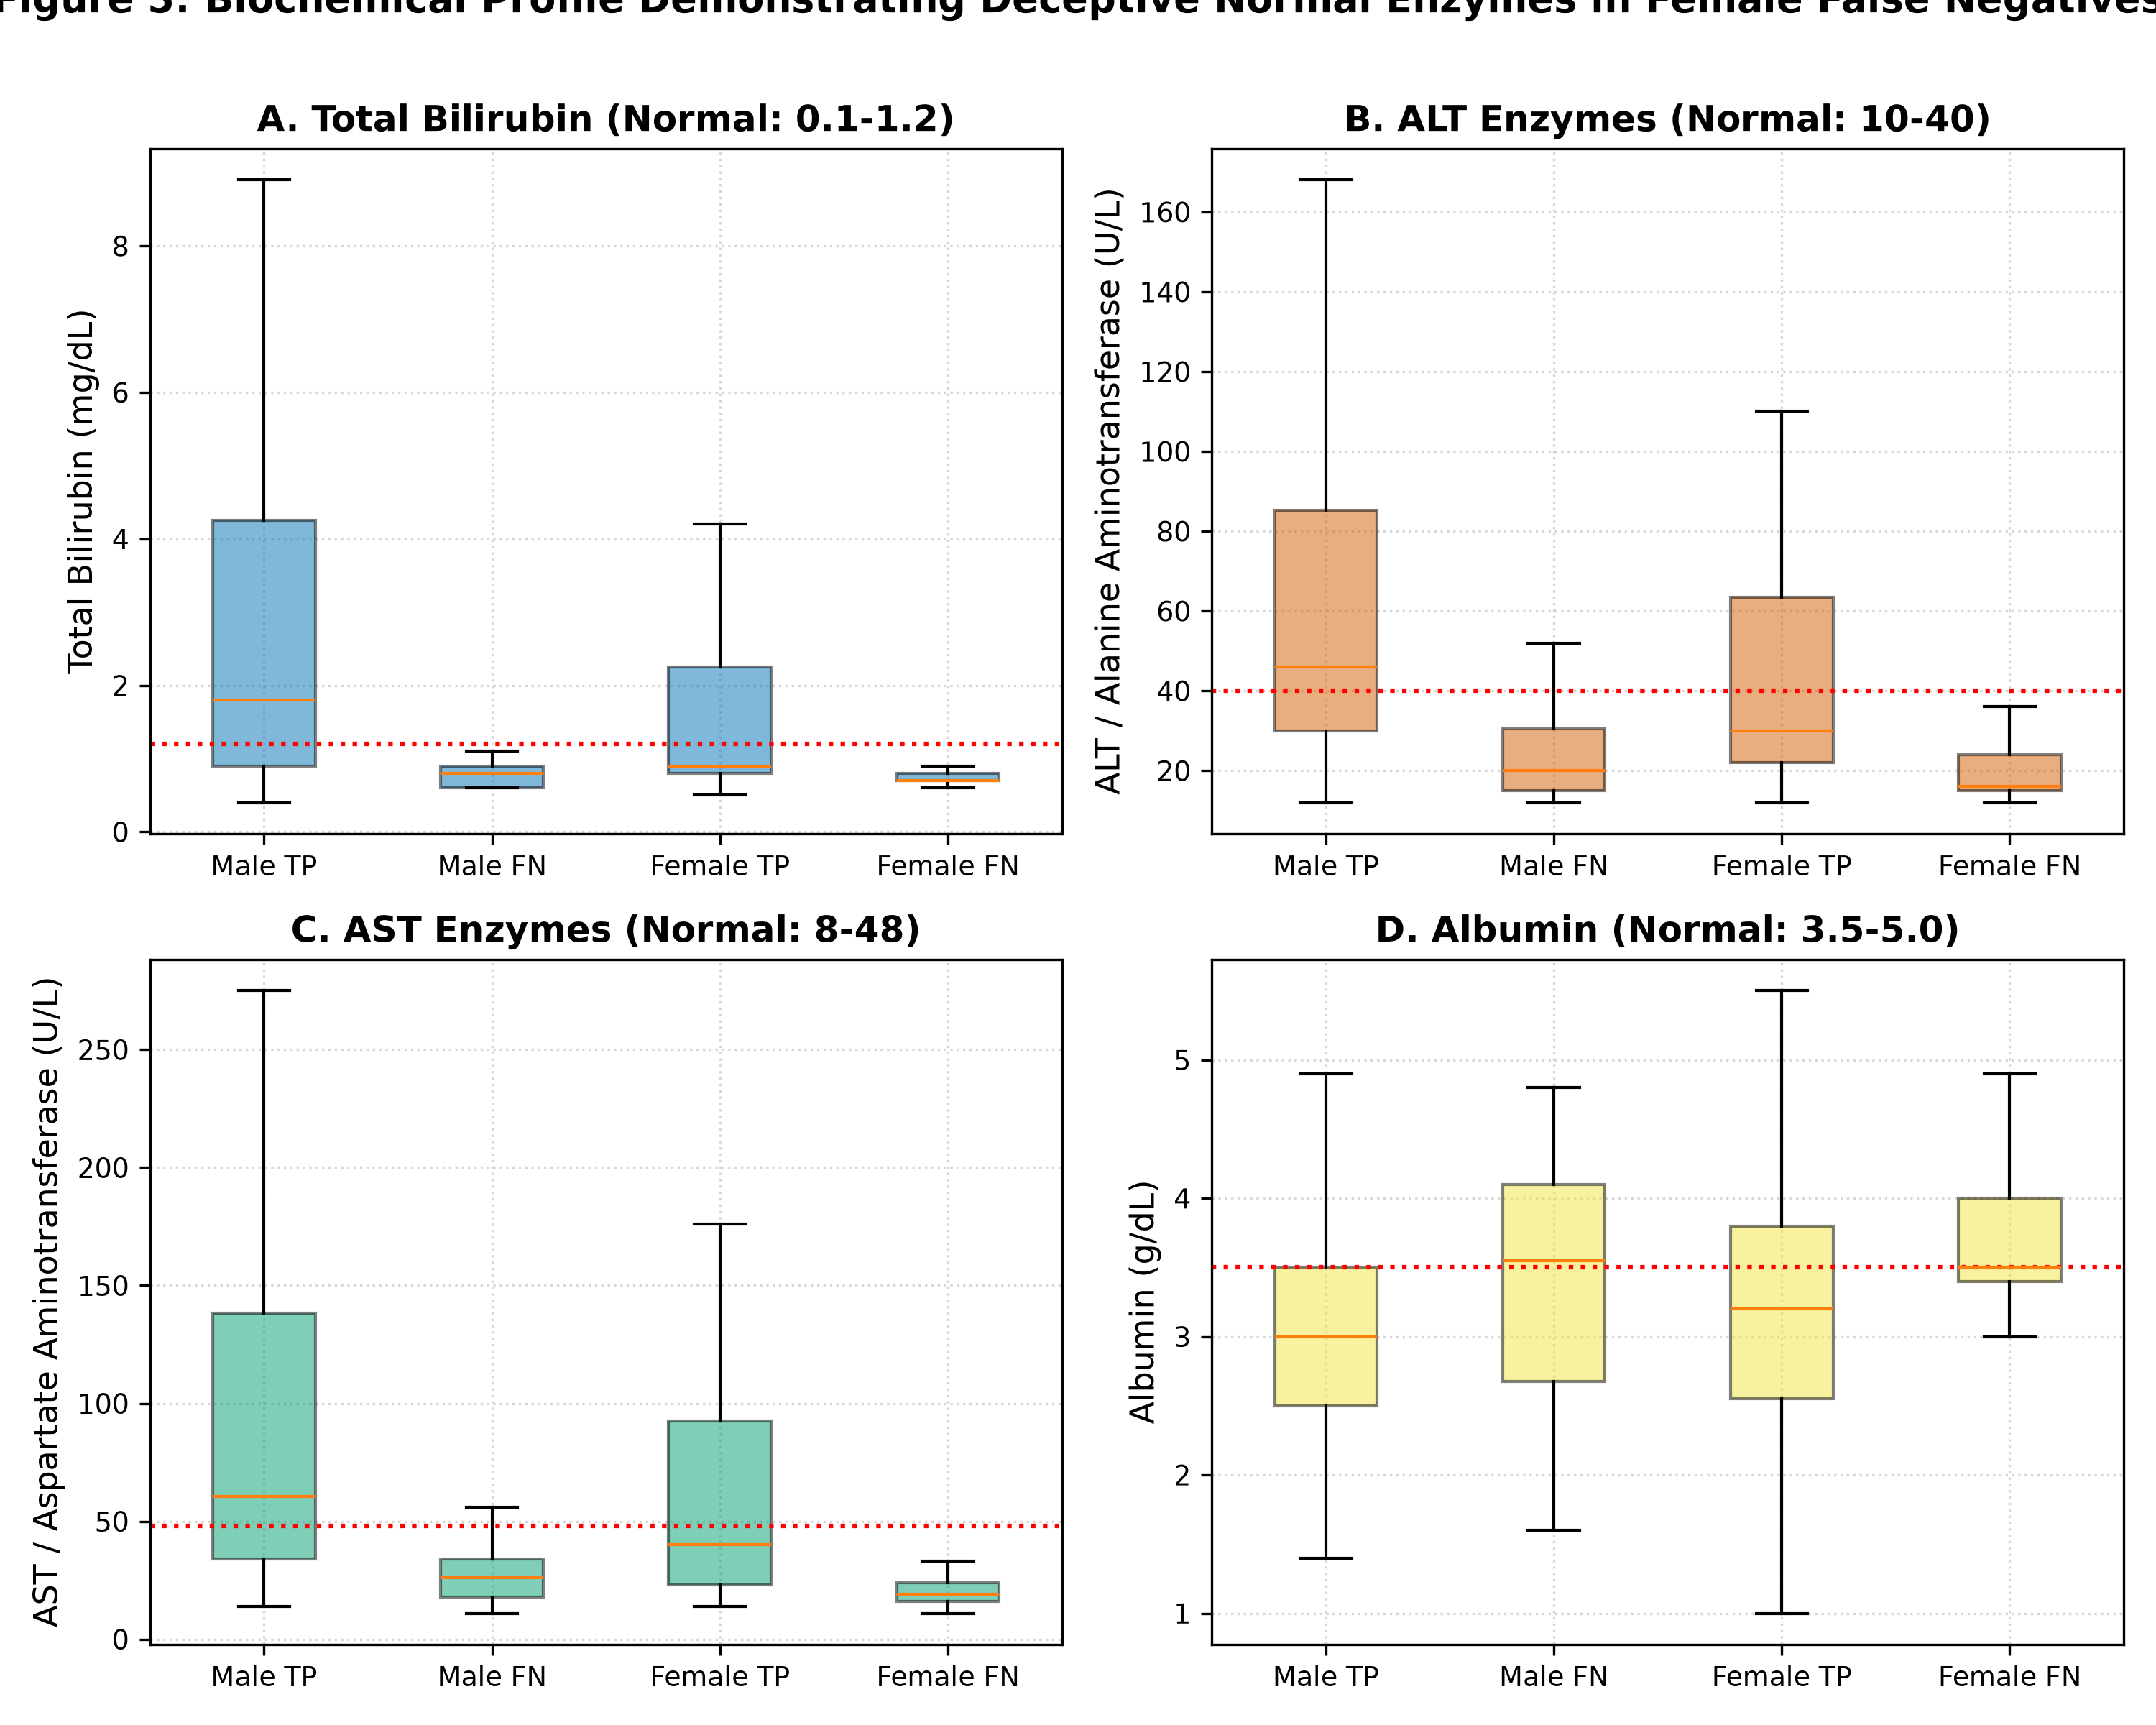
\includegraphics[width=\textwidth]{figures/fig5_false_negative_profile.png}
        \caption{Biomarker profiles of missed disease cases.}
        \label{fig:false_negative_profile}
    \end{subfigure}
    \caption{Model interpretability and false-negative profiling. (a) Standardized odds ratios with 95\% CIs. (b) False negatives in females present with deceptive normal median enzymes compared to males.}
    \label{fig:interpretability_figures}
\end{figure*}

\noindent\textbf{Clinical Anatomy of Female False Negatives:} Out of 33 false-negative predictions at $t^* \approx 0.50$, 13 were female (female share 39.4\%, compared to 24.4\% cohort share). As illustrated in Figure~\ref{fig:false_negative_profile}, female false negatives present with deceptive, clinically normal enzymes: median Total Bilirubin of 0.70 mg/dL (reference: 0.1--1.2 mg/dL) and median ALT of 16.0 U/L (reference: 7--35 U/L). In contrast, male false negatives exhibited elevated median ALT of 48.0 U/L. This biological disparity explains why linear models miss female pathology and justifies sex-aware triage thresholds.

\begin{figure*}[htbp]
    \centering
    \begin{subfigure}[b]{0.48\textwidth}
        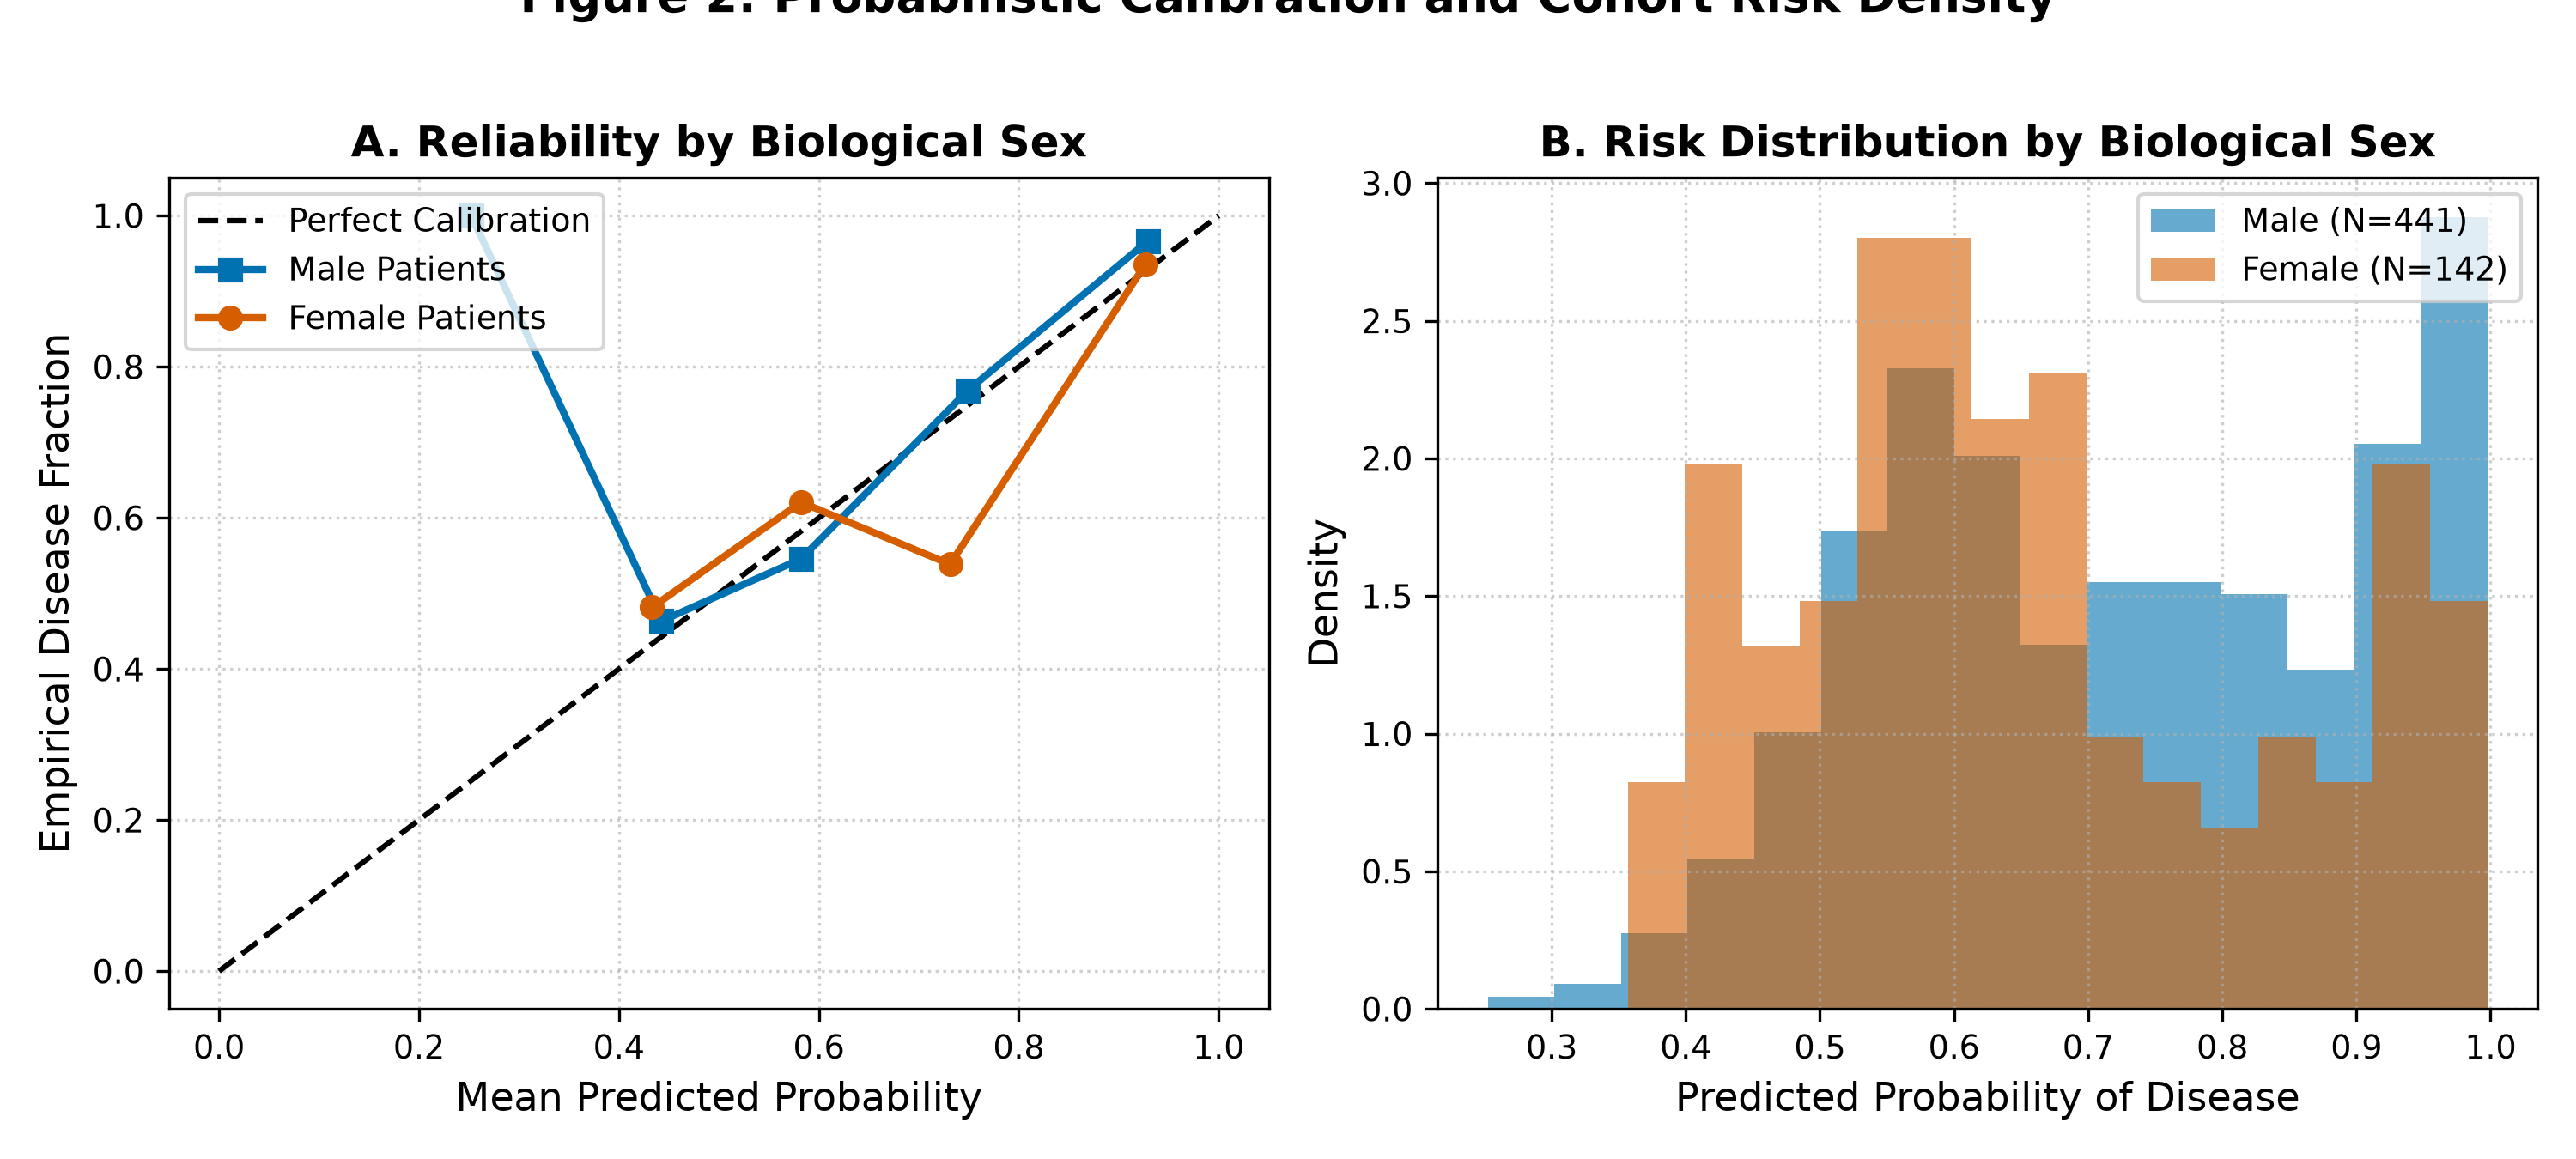
\includegraphics[width=\textwidth]{figures/fig2_calibration_curves.png}
        \caption{Holdout calibration before and after triage.}
        \label{fig:calibration}
    \end{subfigure}
    \hfill
    \begin{subfigure}[b]{0.48\textwidth}
        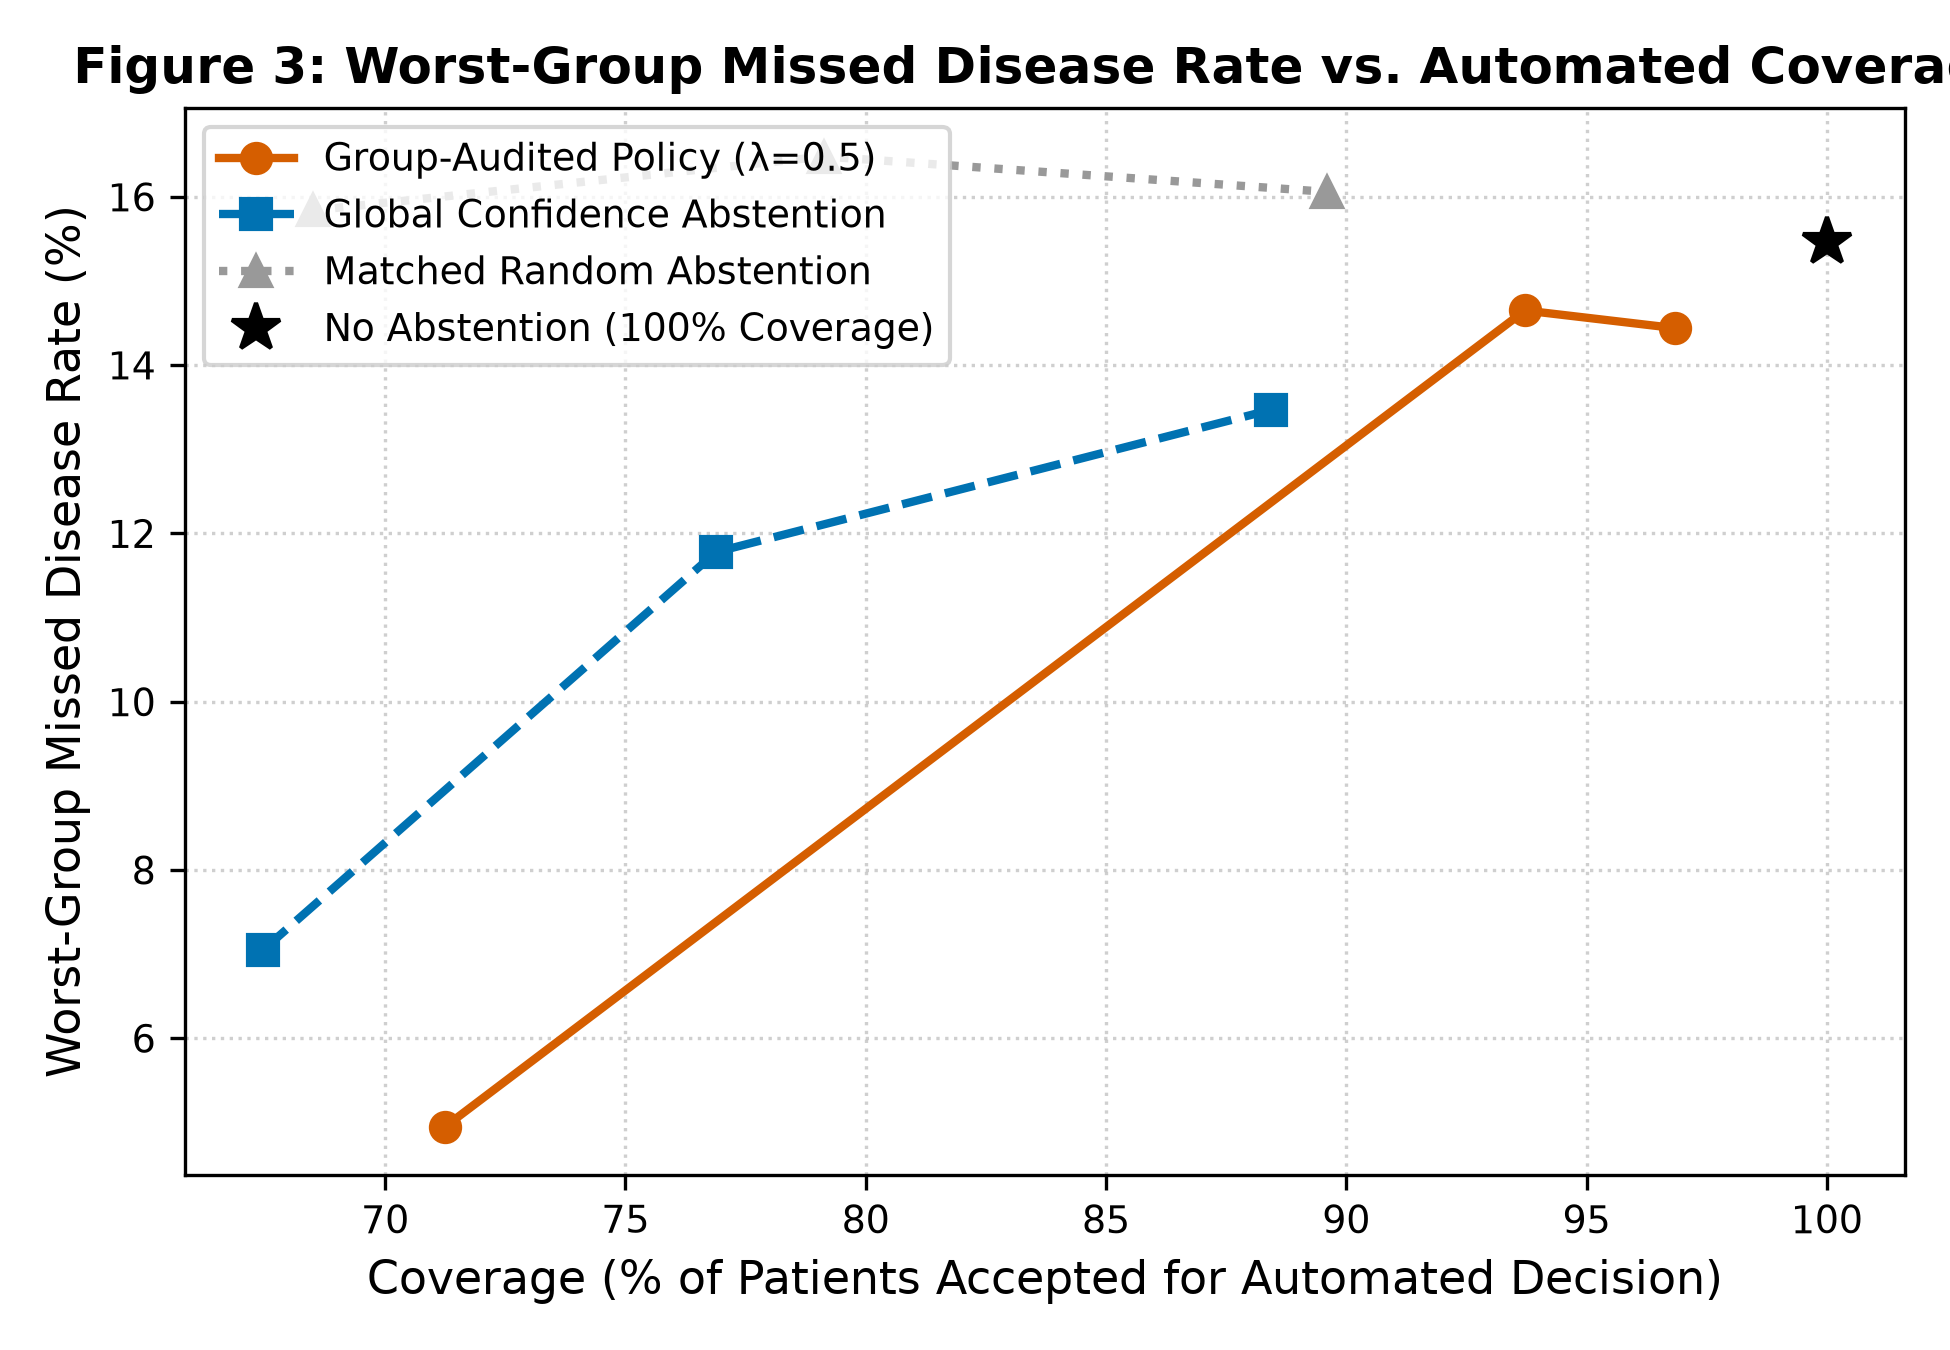
\includegraphics[width=\textwidth]{figures/fig3_risk_coverage.png}
        \caption{Selective risk-coverage curves.}
        \label{fig:risk_coverage}
    \end{subfigure}
    \caption{Calibration and risk-coverage dynamics. (a) Sigmoid calibration preserves reliability across sexes. (b) Monotonically declining selective risk as coverage decreases.}
    \label{fig:dynamics_figures}
\end{figure*}

\section{Discussion \& Limitations}

\subsection{Principal Findings}
Our findings establish three practical conclusions for clinical machine learning:
\begin{enumerate}
    \item Strict nested cross-validation and patient-level bootstrap testing eliminate phantom performance claims and invalid statistical significance.
    \item Operating at a high-sensitivity clinical screening threshold ($91.2\%$ recall) in small-sample liver cohorts inherently yields low specificity ($\approx 23\%$), demonstrating that naive binary classification incurs an overwhelming false-positive burden without selective triage.
    \item The pre-registered primary confirmatory hypothesis ($H_1$) was \textbf{not supported} at $B=0.20$ ($\Delta = -0.47\%$, $p=0.8680$). While sex-audited thresholds reduce worst-group missed disease from 15.5\% to 5.0\% at $B=0.30$, this finding is strictly exploratory vs.\ unbudgeted no-abstention, and finite subgroup sizes ($n=142$ females) constrain statistical power in small-sample cohorts.
\end{enumerate}

\subsection{Limitations (PROBAST+AI Alignment)}
In alignment with our PROBAST+AI self-assessment (\texttt{/paper/PROBAST\_self\_assessment.md}), we declare this study to have an overall \textbf{High Risk of Bias} due to study design constraints:
\begin{itemize}
    \item \textbf{Small Retrospective Convenience Cohort:} The ILPD represents a single regional center in southern India with unknown referral patterns.
    \item \textbf{Absence of Histological Gold Standard:} Diagnoses reflect retrospective clinical classification rather than universal biopsy confirmation.
    \item \textbf{Unmeasured Clinical Referral Costs:} Referral budgets are modeled as mathematical percentages; actual health system economic costs and clinician review burdens were unmeasured.
    \item \textbf{Binary Sex Categorization:} Biological sex was recorded strictly as binary (M/F); hormonal status and gender identity were unrecorded.
    \item \textbf{Calibration $\neq$ Conformal Coverage:} While sigmoid calibration yields reliable probabilities, finite-sample guarantees require transductive split conformal prediction.
\end{itemize}

\section{Reproducibility, Ethics \& Open Science}
All data sources are publicly available under Creative Commons Attribution 4.0 International (CC BY 4.0) licenses. The study adheres to the TRIPOD+AI reporting guidelines (\texttt{/paper/TRIPOD\_AI\_checklist.md}). All code, pinned environment configurations (\texttt{requirements.txt}), random seeds (Seed 42), and cross-validation splits are available open-source. Every number in this manuscript traces directly to reproducible JSON artifacts verified via \texttt{src/verify\_paper\_numbers.py}.

\section{Conclusion}
Small-sample retrospective clinical AI requires methodological rigor to prevent over-optimism and demographic disparities. In this investigation, the pre-registered primary confirmatory hypothesis was \textbf{not supported} at referral budget $B=0.20$, and the high-recall screening setting inherently gives $\approx 23\%$ specificity without selective referral. While referral-budgeted, sex-audited triage provides a principled mechanism to audit and structure clinical trade-offs, and an expanded $B=0.30$ budget achieved a 5.0\% worst-group missed rate, this reduction remains exploratory against no-abstention and requires prospective validation in adequately powered multi-center cohorts.

\bibliographystyle{plain}
\bibliography{references}

\end{document}
